\chapter{The Gram-Schmidt process}

The Gram-Schmidt process takes a set of vectors and provides an orthonormal set of basis vectors. This process has two primary uses in the \svdp:
\begin{enumerate}
\item To build an orthonormal basis for a null space given a set of vectors in the image;
\item To orthonormalize the set of null space vectors output from a matrix reduction.
\end{enumerate}

%%
\section{Process schematic}
Start with a set of $k$ $\mv$s
\begin{equation}
  U = \lst{u_{1},u_{2},\dots,u_{m}}, \quad k\le m.
\end{equation}
If $j$ vectors are linearly independent, the Gram-Schmidt process will produce a set of $j$ orthonormal vectors
\begin{equation}
  V = \lst{\hat{v}_{1},\hat{v}_{2},\dots,\hat{v}_{j}}, \quad j\le k.
\end{equation}

A sample set input and output for two linearly independent vectors is shown in table \eqref{tab:gs:io}. The input set $U$ is shown on the left and the set $V$ is shown on the right. Part of the unit circle is included to show the effect of dilations upon the vectors. The Gram-Schmidt orthogonalization process is then displayed pictorially in the following table \eqref{tab:gs:guts}.

\begin{table}[htdp]
\caption{The Gram-Schmidt orthogonalization depicted for a set of two vectors. The input is the set of $u$ vectors on the left, the output are the orthonormal unit vectors $\hat{v}$ on the right. The vectors are plotted against the upper half of the unit circle to show the effect of dilations.}
$$
\boxed{
\begin{array}{ccc}
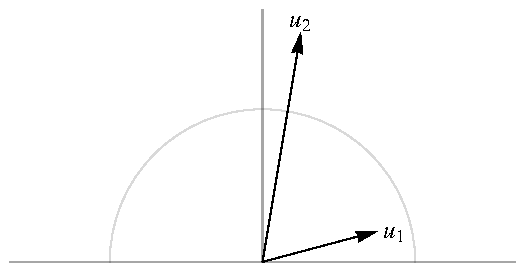
\includegraphics[ width = 2.25in ]{pdf/gs/gs_00.pdf} &
\Rightarrow &
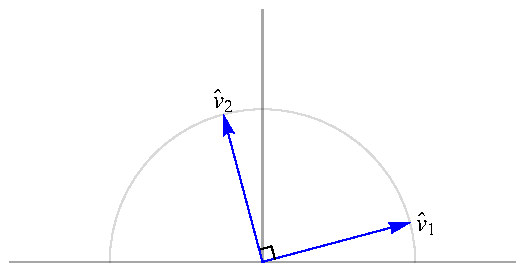
\includegraphics[ width = 2.25in ]{pdf/gs/gs_05.pdf}
\end{array}
}
$$
\label{tab:gs:io}
\end{table}
%%%%
\begin{table}[top]
\caption{The Gram-Schmidt orthogonalization process is detailed for the two input vectors in the previous table. Pick an ordering to sweep through the set of vectors since the process is order dependent. The first action is to normalize the length of the first vector as shown in step 1. Find the orthogonal projection of the second vector onto the first vector. This projection is shown with the red arrow in step 2. For the next step, subtract this projection from the second vector which ``straightens up'' this vector as shown in step 3. Finally, normalize the new vector as shown in step 4.}
$$
\boxed{
\begin{array}{cc}
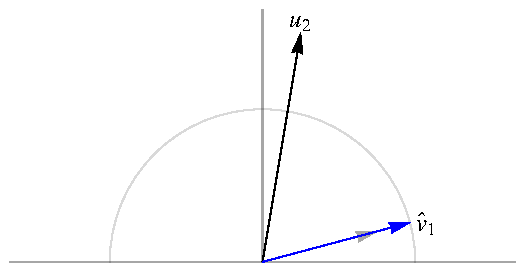
\includegraphics[ width = 2.25in ]{pdf/gs/gs_01.pdf} &
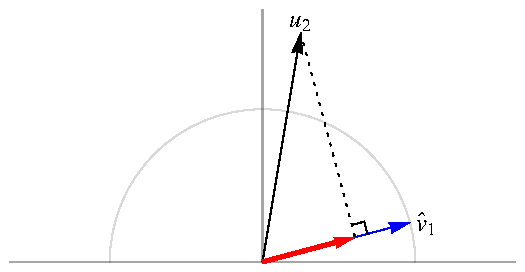
\includegraphics[ width = 2.25in ]{pdf/gs/gs_02.pdf} \\
\text{Step 1: normalization of $v_{1}$.} &
\text{Step 2: projection onto $v_{1}$.} \\[10pt]\hline
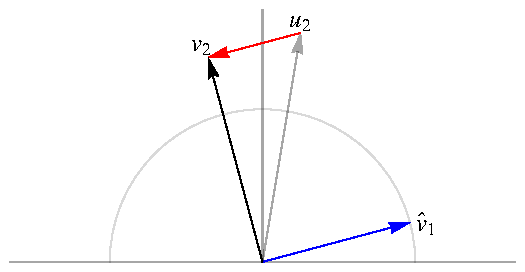
\includegraphics[ width = 2.25in ]{pdf/gs/gs_03.pdf} &
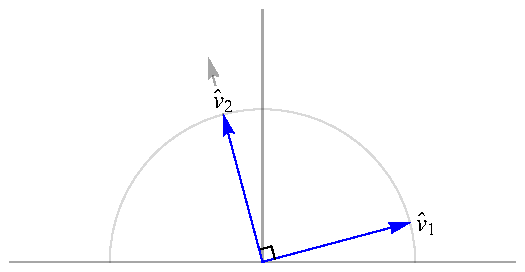
\includegraphics[ width = 2.25in ]{pdf/gs/gs_04.pdf} \\
\text{Step 3: subtract projection.} &
\text{Step 4: normalization of $v_{2}$.}
\end{array}
}
$$
\label{tab:gs:guts}
\end{table}

%%
\section{Projections}
The language of projections is a natural choice for a discussion of the Gram-Schmidt process as one may surmise from the previous table. Recall that the projection of a vector $y$ onto the vector $x$ is defined this way
\begin{equation}
  \pee{}_{x}(y) = \frac{y\cdot x}{x\cdot x}y.
\end{equation}
This notation allows for a compact and intuitive representation of the orthogonalization.

In two dimensions orthogonalization is simple. The generalization to higher dimensions looks follows here. Start with a list with a total of $m$ vectors $U$ in arbitrary ordering. The output will be a set of $n$ orthogonal vectors $V$ which depends upon the ordering of the vectors in the input set. The first few steps look like this:
\begin{equation}
  \begin{array}{cccccccccc}
    v_{1} &=& u_{1}\\
    v_{2} &=& u_{2} &-& \pee{}_{v_{1}}(u_{2})\\
    v_{3} &=& u_{3} &-& \pee{}_{v_{1}}(u_{3}) &-& \pee{}_{v_{2}}(u_{3})\\
    v_{4} &=& u_{4} &-& \pee{}_{v_{1}}(u_{4}) &-& \pee{}_{v_{2}}(u_{4}) &-& \pee{}_{v_{3}}(u_{4})\\
     & \vdots
  \end{array}
\end{equation}
The general formula takes the compact form
\begin{equation}
  v_{k} = u_{k} - \sum_{j}^{m-1}{\pee{}_{v_{j}}(u_{k})}.
\end{equation}

If the vectors in the collection $U$ are linearly independent, then the collection $V$ will have the same number of vectors. That is, $m=n$. If the input vectors have linear dependencies then there will be fewer vectors in the output list and $m>n$. For this discussion only nonzero vectors are relevant.
 
At this juncture the vectors in the set $V$ are orthogonal, but not yet orthonormal. To normalize them use the prescription
\begin{equation}
  \hat{v}_{k} = \frac{v_{k}}{\normt{v_{k}}}, \quad k=1,n.
\end{equation}


%%
\section{Application}
Practice by using the Gram-Schmidt process to compute a few \svdl s.

%%
\subsection{Example 1}

%%
\subsection{Example 2}



\endinput